\begin{document}
\lecture{Implementierung von Datenbanksystemen}{IDB}
\title{Übungsblatt~12}
\subtitle{Planoperatoren}
\maketitle

\begin{note}
	Achtung: Die Angabe von Blatt 13 enthält die Kostenformeln, die in diesem Blatt erarbeitet werden.
	Blatt 13 sollte deshalb erst nach den Übungen zu Blatt 12 herausgegeben werden.
\end{note}

\section*{Lernziele}

\begin{itemize}
  \item Erstellung und algebraische Optimierung von Ausführungsplänen mit Sichten
  \item Optimierung in der Praxis
\end{itemize}

\section*{Literatur}

\HaerderNintyNine{11, 12}

\ElmasriSeventh{18, 19}

\GarciaMolinaSecond{8, 15, 16}

\NeumannFifteen


\section{Fragen zur Vorlesung}

\begin{enumerate}[a)]
	\item Was ist die Aufgabe der Anfrageverarbeitung?

	\begin{solution}
	Abbildung von mengenorientierten Operationen auf effiziente satzorientierte Operationen.
	D.\,h.\ von oben kommen nun keine Satzoperationen mehr, sondern mengenorientierte (Relationenalgebra, SQL).
	Das verringert oft den Programmieraufwand (Beispiel: Mitarbeiter und Abteilungen, VL 10-22).
	Außerdem ist es einfacher zu optimieren.
	Insbesondere muss bei Änderungen an Kardinalitäten etc.\ nicht die Programmstruktur geändert werden.
	Das macht der Optimierer für uns.
	\end{solution}

	\item Aus welchen Schritten besteht sie?

	\begin{note}
	Bild an die Tafel.\\
	Oracle macht das übrigens so 	\url{https://docs.oracle.com/database/121/TGSQL/tgsql_sqlproc.htm\#TGSQL175}
	\end{note}
	\beamertxt{\pagebreak}

	\begin{solution}
	Siehe Folien~\Anfrageverarbeitung.

	Härder:
		Parser macht lexikalische und syntaktische Analyse.
		Semantische Analyse wird bereits mit der Interndarstellung gemacht.
		Das sind Namensauflösung und Typumwandlung.
		Zugriffs- und Integritätskontrolle sind eine Erweiterung der semantischen Analyse.
		"`Standardisierung und Vereinfachung"' und "`Restrukturierung und Transformation"' sind gemeinsam die Optimierung.
	\end{solution}

	\item Angenommen eine Anfrage wird mit gleichen Parametern erneut ausgeführt: Welche Schritte könnten unter welchen Bedingungen eingespart werden?

	\begin{solution}
	Das ist schwieriger, als man denkt:
\begin{itemize}
	\item Sollten sich die Daten nicht geändert haben, könnte man das selbe Ergebnis zurückgeben.
	\item Wenn sich die Daten nur leicht ändern, müsste man nur die Ausführung erneut durchführen, da sich ein anderes Ergebnis ergibt.
	\item Ändern sich die Daten stark, so muss auch die Optimierung erneut durchgeführt werden.
	\item Ändern die Berechtigungen, so muss die Zugriffskontrolle erneut durchgeführt werden.
\end{itemize}
	Rein theoretisch kann man diese Fälle feststellen (Jedes Grant/Revoke prüfen; Statistiken für den Optimierer werden nur explizit geändert, dann kann man prüfen.),
	jedoch wird in der Praxis mit wenigen Ausnahmen einfach die gesamte Anfrageverarbeitung erneut durchgeführt.
	Eine Ausnahme bilden explizit gespeicherte Prozeduren und Funktionen (z.b. PL/SQL).
	\end{solution}

	\item Nun mit unterschiedlichen Parametern.

	\begin{solution}
	Zusätzlich zu den obigen Schritten muss nur die Typkonversion erneut durchgeführt werden.
	Sinnvoll kann zusätzlich eine erneute Optimierung sein ($\mathrm{Wert} > 10$; $\mathrm{Wert} > 1000000$).
	\end{solution}
\end{enumerate}
\begin{beamerText}
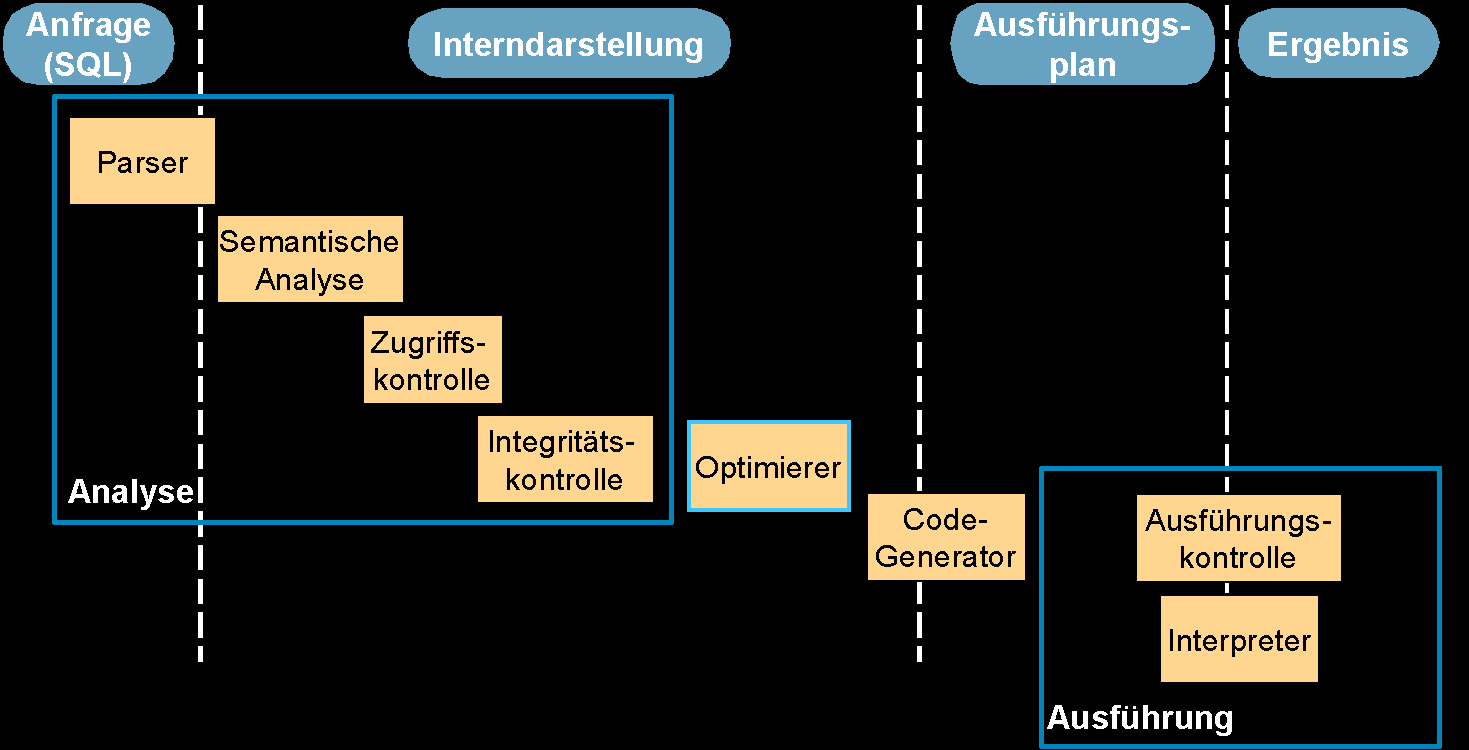
\includegraphics[width=1\linewidth]{Pictures/U10-Beamer-Anfrageverarbeitung}
\pagebreak
\end{beamerText}


\beamertxt{\pagebreak}
\section{Sort-Merge Join}
\label{sec:sort_merge}

\begin{enumerate}[a)]

\item \label{item:sortierung} Entwerfen Sie einen einfachen Algorithmus, der eine Relation sortiert.
	Denken Sie daran, dass der Inhalt der Relation im Allgemeinen nicht komplett in den Puffer passt.
	Geben Sie auch an, wie viele Blockzugriffe auf den Hintergrundspeicher für die Sortierung benötigt werden.

	\begin{solution}
		Die Grundidee besteht darin, Teillisten zu sortieren und diese anschließend zusammenzuführen (Merge).
		Seien \(R\) die zu sortierende Relation mit \(B(R)\) Blöcken und \(M\) die Anzahl verfügbarer Kacheln im Puffer.
		Dann kann \(R\) mit folgendem Algorithmus sortiert werden:

		\begin{enumerate}[1.]
		\item Lies die ersten \(M\) Blöcke von \(R\) in den Puffer.
		\item Sortier diese Blöcke mit einem Hauptspeicher-Sortieralgorithmus.
		\item Schreib die sortierten Blöcke zurück auf den Hintergrundspeicher.
		\item Wiederhol die Schritte 1 bis 3 für alle \(B(R)\) Blöcke.
		\item Reservier eine Kachel für das Ergebnis.
		\item Lies den ersten Block jeder sortierten Teilliste in den Puffer.
		\item Lies das kleinste Elemente der Blöcke im Puffer, füg es in den Ausgabeblock ein.
		\item Schreib den Ausgabeblock auf den Hintergrundspeicher, sobald er voll ist.
		\item Wenn ein Eingabeblock komplett verarbeitet wurde, lade den nächsten Block der Teilliste in den Puffer.
		\end{enumerate}

		Zahl der Blockzugriffe: \(4 B(R)\)
		Falls die sortierten Tupel gleich weiterverarbeitet werden, spart das das Schreiben des Ergebnisses auf den Hintergrundspeicher und somit \(B(R)\) Blockzugriffe.
		Das behandeln wir in \PipeliningKosten genauer.

		In der Praxis passen die ersten Blöcke aller Teillisten meistens in den Hauptspeicher.
		Sollte das nicht der Fall sein, kann eine weitere Merge-Phase angehängt werden.
	\end{solution}

\item Wie viele Blockzugriffe werden für die Durchführung eines Sort-Merge Joins von zwei Relationen \(R\) und \(S\) insgesamt benötigt, wenn zur Sortierung der Algorithmus aus Teilaufgabe \ref{item:sortierung}) und für die anschließende Durchführung des Merge Joins der in der Vorlesung (Folie~\MergeJoin) vorgestellte Algorithmus verwendet werden?

	\begin{solution}
		Die sortierten Relationen müssen schritthaltend jeweils einmal gelesen und das Ergebnis muss wieder abgelegt werden.
		Somit ergibt sich eine Gesamtzahl von \(6 (B(R) + B(S))\) Blockzugriffen.
		Äquivalent zur Sortierung spart die direkte Weiterverarbeitung der Join-Ergebnisse \(B(R) + B(S)\) Blockzugriffe.

		Für den Merge braucht man normal nur zwei Pufferkacheln.
		Sollte sich aber ein Wert eines Join-Attributs über mehrere Blöcke erstrecken, so müssen all diese Blöcke gleichzeitig in den Puffer gelesen werden.
		Für den Fall, dass dafür nicht genügend Kacheln zur Verfügung stehen, muss für die Tupel mit diesem Wert ein One-Pass Join oder ein Nested-Loop Join durchgeführt werden.
	\end{solution}

\item \label{item:kombiniert}Überlegen Sie, wie die Algorithmen aus den vorherigen beiden Teilaufgaben kombiniert werden können, um Blockzugriffe einzusparen.
	Welche Voraussetzungen müssen die am Join beteiligten Relationen dafür erfüllen?

	\begin{solution}
		\begin{enumerate}[1.]
		\item Führ die Schritte 1 bis 4 des Sortieralgorithmus für beide Relationen aus.
		\item	Lies den ersten Block jeder Teilliste beider Relationen in den Puffer.
		\item Such den niedrigsten Wert des Join-Attributs in allen Tupeln aller Blöcke im Puffer und join die Tupel mit dem gleichen Wert.
		\end{enumerate}

		Damit werden nur noch \(4 (B(R) + B(S))\) Blockzugriffe bzw.\ bei direkter Weiterverarbeitung \(3 (B(R) + B(S))\) Blockzugriffe benötigt.

		Voraussetzung für diesen Algorithmus ist, dass beide Relationen zusammen weniger Teillisten haben, als Hauptspeicherkacheln zur Verfügung stehen.
		Da jede Teilliste maximal \(M\) Blöcke enthält, muss gelten \( \left \lceil \frac{B(R)}{M} \right \rceil + \left \lceil \frac{B(S)}{M} \right \rceil < M\).
		Bei vielen gleichen Werten des Join-Attributs ist wie bei der nicht-optimierten Variante ein besonderes Vorgehen notwendig.
	\end{solution}
\end{enumerate}


\beamertxt{\pagebreak}
\section{Sort-Merge Join in der Anwendung}

Gegeben sind zwei Relationen A und B mit jeweils zwei Attributen ax und ay bzw.\ bx und by.
Das Attribut by ist als UNIQUE gekennzeichnet.

\begin{center}
	\begin{minipage}{5cm}
		\begin{center}

			\textbf{Relation A}
			\begin{tabular}{|p{2cm}|p{2cm}|}
				\hline
				\textbf{ax} & \textbf{\textit{ay}} \\\hline
				1 & 11 \\\hline
				2 & 18 \\\hline
				4 & 5 \\\hline
				8 & 9 \\\hline
				16 & 1337 \\\hline
				32 & 9 \\\hline
				64 & 32 \\\hline
				128 & 42 \\\hline
				265 & 18 \\\hline
				512 & 58 \\\hline
				1024 & 11 \\\hline
				2048 & 55 \\\hline
			\end{tabular}

		\end{center}
	\end{minipage}
	%
	\hspace{2cm}
	%
	\begin{minipage}{5cm}
		\begin{center}

			\textbf{Relation B}
			\begin{tabular}{|p{2cm}|p{3cm}|}
				\hline
				\textbf{bx} & \textbf{\textit{by} (UNIQUE)} \\\hline
				12 & 9 \\\hline
				3 & 42 \\\hline
				6 & 11 \\\hline
				10 & 18 \\\hline
			\end{tabular}

		\end{center}
	\end{minipage}
\end{center}

Führen Sie einen Inner Join mit der Bedingung \emph{A.ay = B.by} mittels Sort-Merge Join durch. Im Puffer stehen 5 Kacheln zur Verfügung. Gehen Sie zur Vereinfachung davon aus, dass pro Block jeweils nur ein Tupel abgelegt ist.

Geben Sie die einzelnen Schritte und Zwischenergebnisse des Algorithmus an: Geben Sie zu jedem Schritt den Zustand und die Änderungen im Hauptspeicher an (z.\,B.\ "`Aus Relation A drittes Tupel in Kachel 1 und fünftes Tupel in Kachel 2 laden"'). Geben Sie außerdem die Änderungen an der Ergebnisrelation nach dem jeweiligen Schritt an.

\begin{solution}
	Lade A1-A5: Sortiert speichern in C (Neue Liste), Reihenfolge: A3, A4, A1, A2, A5\\
	Lade A6-A10: Sortiert speichern in D (Neue Liste), Reihenfolge: A6, A9, A7, A8, A10\\
	Lade A11-A12: Sortiert speichern in E (Neue Liste), Reihenfolge: A11, A12\\
	Lade B1-B4: Sortiert speichern in F (Neue Liste), Reihenfolge: B1, B3, B4, B2

	Zuordnung: C in Kachel 1, D in Kachel 2, E in Kachel 3, F in Kachel 4

	\hspace{-2.3cm}\begin{tabular}{|cc|cc|cc|cc|c|}
		\hline
		\textbf{Kachel 1} &   & \textbf{Kachel 2} &  & \textbf{Kachel 3} & & \textbf{Kachel 4} & & \textbf{Kachel 5} \\
		\hline
		\cellcolor{orange} C1 = A3 & (4, 5) & D1 = A6 & (32, 9) & E1 = A11 & (1024, 11) & F1 = B1 & (12, 9) &  \\
		\hline
		\cellcolor{orange}\underline{C2 = A4} & (8, 9) & D1 = A6& (32, 9) & E1 = A11 & (1024, 11) & \underline{F1 = B1} & (12, 9) & (8, 9, 12, 9)\\
		\hline
		C3 = A1 & (1, 11) & \cellcolor{orange}\underline{D1 = A6}& (32, 9) & E1 = A11 & (1024, 11) & \underline{F1 = B1} & (12, 9) &(32, 9, 12, 9) \\
		\hline
		C3 = A1 & (1, 11) & D2 = A9 & (265, 18) & E1 = A11 & (1024, 11) & \cellcolor{orange} F1 = B1 & (12, 9) &  \\
		\hline
		\cellcolor{orange}\underline{C3 = A1} & (1, 11) & D2 = A9 & (265, 18) & E1 = A11 & (1024, 11) & \underline{F2 = B3} & (6, 11) & (1, 11, 6, 11)\\
		\hline
		C4 = A2 & (2, 18) & D2 = A9 & (265, 18) & \cellcolor{orange}\underline{E1 = A11} & (1024, 11) & \underline{F2 = B3} & (6, 11) & (1024, 11, 6, 11) \\
		\hline
		C4 = A2 & (2, 18) & D2 = A9 & (265, 18) & E2 = A12 & (2048, 55) & \cellcolor{orange}F2 = B3 & (6, 11) & \\
		\hline
		\cellcolor{orange}\underline{C4 = A2} & (2, 18) & D2 = A9 & (265, 18) & E2 = A12 & (2048, 55) & \underline{F3 = B4} & (10, 18) & (2, 18, 10, 18)\\
		\hline
		C5 = A5 & (16, 1337) & \cellcolor{orange} \underline{D2 = A9} & (265, 18) & E2 = A12 & (2048, 55) & \underline{F3 = B4} & (10, 18) & (265, 18, 10, 18)\\
		\hline
		C5 = A5 & (16, 1337) & D3 = A7 & (64, 32) & E2 = A12 & (2048, 55) & \cellcolor{orange}F3 = B4 & (10, 18) & \\
		\hline
		C5 = A5 & (16, 1337) &\cellcolor{orange} D3 = A7 & (64, 32) & E2 = A12 & (2048, 55) & F4 = B2 & (3, 42) & \\
		\hline
		C5 = A5 & (16, 1337) &\cellcolor{orange}\underline{D4 = A8} & (128, 42) & E2 = A12 & (2048, 55) & \underline{F4 = B2} & (3, 42) & (128, 42, 3, 42)\\
		\hline
		C5 = A5 & (16, 1337) &D5 = A10 & (512, 58) & E2 = A12 & (2048, 55) & \cellcolor{orange}F4 = B2 & (3, 42) &\\
		\hline
		C5 = A5 & (16, 1337) &D5 = A10 & (512, 58) & E2 = A12 & (2048, 55) &  &  &
		\\
		\hline
	\end{tabular}

Abbruch, da keine weiteren Kombinationen mehr möglich sind.

\paragraph{\color{solutioncolor}Hinweis:} \begin{tabular}{|c|}
		\hline
		\cellcolor{orange}\\
		\hline
	\end{tabular}
bedeutet, dass dieser Slot im nächsten Schritt neu eingelesen wird. \\
	\underline{Der Unterstrich} weist darauf hin, dass dieser Slot in diesem Schritt mit einem anderen kombiniert wird.
\end{solution}


\beamertxt{\pagebreak}
\section{Kosten der Operatorausführung}
\label{sec:kosten}

\begin{enumerate}[a)]

\item Bei einer kostenbasierten Optimierung stellen die Kosten die Größe dar, die minimiert werden soll.
	Welche Werte könnte man bei der Optimierung von Datenbankanfragen in die Kosten einfließen lassen?

	\begin{solution}
		Z.\,B.\ Anzahl Blockzugriffe auf den Hintergrundspeicher, CPU-Zeit, Hauptspeicherbedarf, \ldots
	\end{solution}

\item \label{item:kostenformeln} Wir nehmen ein einfaches Kostenmodell an, das nur die Lese- und Schreibvorgänge auf dem Hintergrundspeicher berücksichtigt.
	Stellen Sie dafür Kostenformeln für die Planoperatoren Selektion, Projektion, Nested-Loop Join, Sort-Merge Join und Hash Join auf.
	Gehen Sie davon aus, dass die Eingaben vom Hintergrundspeicher gelesen werden müssen und die Ergebnisse direkt ausgegeben werden.
	\(B(S)\) gibt die Anzahl der Blöcke an, aus denen die Relation \(S\) besteht.

	\begin{solution}
		\begin{tabular}{l l p{5cm}}
			\hline
			\textbf{Implementierung} & \textbf{Kosten}          &                                                         \\ \hline
			Selektion(S)             & $B(S)$                   &                                                         \\ \hline
			Projektion(S)            & $B(S)$                   &                                                         \\ \hline
			NestedLoopJoin(S, T)     & $B(S) + B(S) \cdot B(T)$ &                                                         \\ \hline
			SortMergeJoin(S, T)      & $3 (B(S) + B(T))$        & Unter den in \SortMergeJoin genannten Voraussetzungen   \\ \hline
			HashJoin(S, T)           & $B(S) + B(T)$            & Classic Hashing, wenn eine Relation in den Puffer passt \\ \hline
		\end{tabular}

		Die Kosten werden einheitslos angegeben, da sie nur zum Vergleich zwischen den Operatoren dienen.

		In der Literatur finden sich je nach verwendetem Kostenmodell und berücksichtigten Kostentypen unterschiedliche Formeln. Eine gute Herleitung von Kostenformeln steht bei Garcia-Molina et al.
	\end{solution}

\item \label{item:pipelining} Pipelining bezeichnet das direkte Hintereinanderausführen mehrerer Operatoren, ohne die Zwischenergebnisse erst komplett zu erzeugen und auf den Hintergrundspeicher zu schreiben.
	Welche der aus der Vorlesung und Übung bekannten Planoperatoren eignen sich für Pipelining gut, welche nicht?

	\begin{solution}
		Als Quelle für Pipelining können alle Operatoren dienen.
		Zu beachten ist dabei aber, dass vom Quelloperator belegte Pufferkacheln nicht für den Zieloperator zur Verfügung stehen.
		Werden Table Scan und Index Scan als eigenständige Operatoren behandelt, wie wir das im Folgenden tun, dann werden sie immer per Pipelining mit dem folgenden Operator verbunden.
		Ein Table-Scan-Operator ohne Pipelining wäre sinnlos, da er lediglich die Relation umkopieren würde.

		Als Ziel für Pipelining sind alle Operatoren gut geeignet, die die Quelle nur einmal durchlaufen müssen, beispielsweise Selektion, Projektion oder auch die äußere Relation des Nested-Loop Joins.

		Der Nested-Loop Join ist gleichzeitig auch ein Beispiel für einen Operator, der sich nicht gut als Ziel für Pipelining eignet.
		Wird die innere Relation nicht zwischengespeichert, muss sie für jeden Durchlauf neu erzeugt werden.
	\end{solution}

\item Wie ändern sich die Kostenformeln aus Teilaufgabe \ref{item:kostenformeln}), wenn Pipelining eingesetzt wird?
Verwenden Sie \(C(S)\) für die Kosten zur Erzeugung der Zwischenergebnisrelation \(S\).

	\begin{solution}
		Dient ein Operator A als Eingabe für einen weiteren Operator B, können dessen Kosten in der Kostenformel für B an der Stelle der Blockzugriffe zum Lesen der Eingaberelation angesetzt werden.
		Blockzugriffe für das Schreiben des Ergebnisses werden nicht benötigt, da das Ergebnis direkt an den nächsten Operator oder an den Anwender weitergegeben wird.
		Die Gesamtkosten einer Anfrage sind dann einfach die Kosten der Wurzel im Operatorbaum.

		Beispiel: Selektion(S) hat mit Pipelining Kosten von C(S). Das bedeutet, dass die Kosten eines Selektionsoperators gerade so hoch sind wie die Erzeugungskosten seiner Eingabedaten. Das liegt daran, dass wir nur E/A-Kosten berücksichtigen und die Selektion selbst keine Ein- oder Ausgabe vornimmt.

		Als Kostenformeln mit Pipelining ergeben sich:

		\begin{tabular}{l l}
			\hline
			\textbf{Implementierung} 	& \textbf{Kosten}\\
			\hline
			Selektion(S)						& $C(S)$\\
			\hline
			Projektion(S)						& $C(S)$\\
			\hline
			TableScan	(S)							& $B(S)$\\
			\hline
			IndexScan(S)							& $a \cdot \left \lceil{ B(S) \cdot \mathrm{Selektivit"atsfaktor} }\right \rceil $\\
			\hline
			NestedLoopJoin(S, T)			& $C(S) + B(S) \cdot C(T)$\\
			\hline
			SortMergeJoin(S, T)				& $C(S) + C(T) + 2 (B(S) + B(T))$\\
			\hline
			HashJoin(S, T) 						& $C(S) + C(T)$\\
			\hline
		\end{tabular}

		Beim Index Scan wurden hier die Kosten eines wahlfreien Blockzugriffs als a-mal so hoch wie die eines sequentiellen Blockzugriffs angesetzt.
	\end{solution}

\end{enumerate}


\begin{deeper}
\section{Programmieraufgabe 8: Metadatenbank}

\subsection{Aufgabenstellung}
\begin{enumerate}
	\item Implementieren Sie eine Klasse, die die Schnittstelle \beamertxt{\linebreak}\texttt{idb.meta.Metadata} implementiert.
		Beachten Sie die Dokumentation der Methoden in der Schnittstelle.
	\item Tragen Sie den Konstruktor Ihrer Klasse in \texttt{idb.construct.Util} in der Methoden \texttt{createMetadata()} ein.
		Diese Methode erhält neben dem \texttt{DBBuffer} einen \texttt{idb.meta.FileCache} und einem Array mit 6 Strings, die als Pfade für beliebige Dateien verwendet werden können.
		Diese Dateien werden beim Aufruf bereits erzeugt und leer sein.
	\item Tragen Sie außerdem einen Konstruktor Ihrer Klasse in \texttt{idb.construct.Util} in der Methode \texttt{reloadMetadata()} ein.
		Diese Methode erhält die selben Parameter wie \texttt{createMetadata}, soll jedoch keine neue Datenbank anlegen, sondern diese wiederherstellen
	\item Sorgen Sie dafür, dass Sie alle Tests aus der Klasse \texttt{MetaTests} erfüllen.
	Sie können diese Testfälle mit \lstinline|ant Meilenstein8a| ausführen.
	\item Sorgen Sie dafür, dass Sie alle Tests aus der Klasse \texttt{LoadedMetaTests} erfüllen.
	Sie können diese Testfälle mit \lstinline|ant Meilenstein8b| ausführen.
	\item Die Abgabe auf GitLab erfolgt zeitgleich mit der Abgabe der Zusatzaufgaben des nächsten Übungsblattes auf StudOn. Markieren Sie hierfür Ihre Abgabe mit dem Tag "`Aufgabe-8"'.
\end{enumerate}

\subsection{Hinweise}
\begin{itemize}
	\item Der \texttt{FileCache} bietet angenehme Methoden zur Produktion von TIDFiles und KeyRecordFiles aus Pfaden.
		Verwenden Sie diese anstelle der in \texttt{idb.construct.Util} von Ihnen eingetragenen Methoden um Probleme mit mehreren (verschiedenen) Instanzen von KeyRecord / TIDFile auf geteilten Dateien zu verhindern.
		Rufen Sie niemals \texttt{close} auf den Dateien aus dem FileCache auf, da dieses für Sie übernommen wird.
	\item Der \texttt{FileCache} ist nicht zur Erzeugung neuer Dateien geeignet. Rufen Sie dafür weiterhin die von Ihnen in \texttt{idb.construct.Util} eingetragenen Funktionen auf.
		Beachten Sie, dass Sie für die selbst generierten und nicht aus FileCache stammenden Blockfiles und KeyRecordFiles selbstständig \texttt{close} aufrufen müssen.
		Um diese Unterscheidung nicht dauerhaft vornehmen zu müssen, hilft es, die erzeugten Dateien schnell zu schließen und dann über den \texttt{FileCache} erneut öffnen zu lassen.
	\item Beachten Sie, dass ein Puffer wie im Clock-Puffer Referenzen auf bereits mit \texttt{unfix} freigegebene Kacheln beibehält, bis die jeweilige Kachel wieder gebraucht wird.
		Wenn Sie nun \texttt{close} auf den Blockfiles aufrufen, geraten Sie bei späteren \texttt{fix} Aufrufen dann in problematische Fehler oder Randfälle.
		Bei einer korrekten Implementierung des Clock-Puffers inklusive des Zurücksetzens von \texttt{setDirty} im \texttt{flush} können Sie mit eben diesem \texttt{flush} dieses Problem umgehen.
		Notfalls können Sie auch testweise im Testfall den Clock-Puffer durch den sehr viel langsameren Simple-Buffer ersetzen, indem Sie die entsprechenden Zeilen im Setup ein- und auskommentieren.
	\item Unsere Indexstrukturen sind ausschließlich als Sekundärstrukturen verwendbar. Aufgrund der Einschränkungen der Hash-Implementierung können diese nicht als Primärstrukturen verwendet werden.
	\item Um unsere in der letzten Aufgabe erstellte Funktion zum Löschen von Tupeln einer Relation zu verwenden, verlangen wir für jede Relation einen Sekundärindex, aufgebaut auf dem Primärschlüssel.
	\item Während es Ihnen freigestellt ist, wie Sie Ihre sechs Dateien verwenden, empfehlen wir zwei Tabellen mit jeweils einer TIDFile und einem Index auf dem Primärschlüssel als KeyRecordFile / LinHash.
	\item Wir empfehlen die folgenden zwei Tabellen: 
\begin{enumerate}
\item Attributes(\textit{Name}: String, \textit{Rel}: String, \textit{Type}: String, \textit{Pos}: Int, \textit{PrimaryKey}: Boolean, \textit{SurrogateKey}: Boolean, \textit{\_Surrogate}: Int): Bei \textit{\_Surrogate} handelt es sich um den Surrogat-Primärschlüssel
\item Files(\textit{Path}: String, \textit{Relation}: String, \textit{Type}: String, \textit{BlockSize}: Int):
\textit{Path} bezeichnet den Primärschlüssel, der \textit{Type}-String kodiert ob es sich um eine \textit{TID-File}, den \textit{Regulärbereich} eines Hashing oder um den \textit{Overflowbereich} des Hashing handelt.
Im Falle einer \textit{Indexdatei} (Hashing, Regulär und Overflow) muss zusätzlich im \textit{Type}-String kodiert werden, welches Attribut in diesem Index als Schlüssel verwendet wird, üblicherweise durch seine (eindeutige) Position in der Relation.
\end{enumerate}
Die Verwendung von zwei Tabellen dieser festen Struktur hat den Vorteil, die Planoperatoren der letzten Aufgabe in der Meta-Datenbank verwenden zu können.
		Im Gegensatz zur echten Datenbank sind hier die Attributnamen und -typen jedoch unveränderlich, sodass die entsprechenden \texttt{NamedCombinedRecord} zur Pogrammierzeit bestimmt werden können.
		Dabei sind die Attribute wie folgt zu verstehen:
		\begin{enumerate}
			\item \textit{Attributes.Name}: Der (in einer Relation eindeutige) Name eines Attributes. Attributnamen bestehen ausschließlich aus den Buchstaben A-Z und a-z.
			\item Attributes.Rel: Der Name der Relation, in dem dieses Attribut definiert sein soll.
			\item \textit{Attributes.Type}: Der Typ des Attributes. In unserer Datenbank entweder \texttt{DBString}, \texttt{Bool} oder \texttt{IntegerKey}. Die Darstellung als String empfiehlt sich einfach zu halten (z.B. durch einen Buchstaben).
			\item \textit{Attributes.Pos}: Die Position dieses Attributes in einem \mbox{NamedCombinedRecord} dieser Relation. Da ein \mbox{NamedCombinedRecord} nicht das Layout speichert, muss dieses in den Metadaten abgelegt werden.
			\item \textit{Attributes.PrimaryKey}: Jede Relation benötigt einen Primärschlüssel.
			\item \textit{Attributes.SurrogateKey}: Unsere Datenbank bietet Nutzern einen Surrogatschlüssel an, den der Nutzer nicht angeben muss, sondern den das DBMS für den Nutzer errechnet und einträgt. Wenn eine Relation einen solchen Surrogatschlüssel verwenden soll, ist dieser Boolean beim PrimaryKey wahr, andernfalls falsch.
			\item \textit{Attributes.\_Surrogate}: Nachdem es keinen sinnvollen Primärschlüssel für die Attributes Relation gibt, soll diese bereits ein Surrogatschlüssel verwenden.
			Der Attributname "\_Surrogate"\ soll generell verwendet werden, wenn ein Surrogatschlüssel angelegt wird, und wird durch die Einschränkung der Attributnamen auch immer zur Verfügung stehen.
			\item \textit{Files.Path}: Der Pfad zu einer Datei.
			\item \textit{Files.Relation}: Der Name der Relation, zu welcher diese Datei gehört.
			\item \textit{Files.Type}: Der bereits beschriebene Typestring der Datei.
			\item \textit{Files.BlockSize}: Die BlockSize, die für diese Datei zu verwenden ist.
				Durch technische Einschränkungen in unserer Datenbank ist diese vermutlich für alle Dateien gleich.
				Jedoch benötigen Sie für das Öffnen der Dateien die BlockSize, und nachdem Sie für den Pfad zur Datei bereits die Files-Relation durchsuchen müssen,
				erhalten Sie durch dieses Attribut diese Information nahezu umsonst.
		\end{enumerate}
	\item Verwenden Sie für die sechs im Konstruktor übergebenen Pfade BlockSize 4096, da andernfalls aufgrund unseres Puffers die Testfälle,
		die eine andere BlockSize für neu zu erzeugende Dateien verlangen, fehlschlagen werden.
	\item Zum Entwickeln der Methoden lohnt es sich, initial ein SQL-Statement auf den zwei Relationen zu formulieren und dann dieses in Planoperatoren umzuwandeln.
		Ein Beispiel: Für \texttt{addRelation} muss überprüft werden, ob eine Relation des Namens \textit{Student} schon existiert. In SQL interessiert uns, ob es für folgende Ausgabe mindestens ein Tupel gibt:
\begin{verbatim}
Select *
From Attributes
Where Attributes.Rel == Student
\end{verbatim}
In unserer Datenbank sähe dies dann so aus:
\begin{verbatim}
Module m = getTableScanAttributes();
m = Util.generateSel(m, x -> x.getString("Rel").equals("Student"));
boolean unused = (m.pull() == null);
m.close();
\end{verbatim}
	\item Falls eine Aggregation ohne Gruppierung verwendet werden soll, kann diese dadurch herbeigeführt werden, zuerst die Tupel durch ein \texttt{generate} zu schicken, in denen jedem Tupel der gleiche Wert zugewiesen wird (mit einem Attributnamen der nicht in der Relation vorkommen kann, z.B. durch die Verwendung eines Unterstrichs).
		Danach kann dieses neue Attribut nun zum Gruppieren verwendet werden und aggregiert damit alle Tupel.
	\item Verwenden Sie für Aggregationen die vorgefertigten Tripel aus \texttt{Util.count}, \texttt{Util.max} oder \texttt{Util.min}.
	\item Verwenden Sie zur Berechnung des Surrogatschlüssels für ein neu einzufügendes Tupel nicht \texttt{Util.count}.
	\item Achten Sie darauf, beim Hinzufügen von Tupeln (sowohl in den Metarelationen als auch in den verwalteten Datenbankrelationen) die Indices mit zu aktualisieren.
	\item Durch die Stabilität von TID ist eine Referenz auf einen bereits gelöschten Datensatz in einem nicht zum Löschen verwendeten Index kein Problem.
			Der Nutzer muss die Reaktion auf Verweise auf gelöschte Sätze selbstständig implementieren.
	\item Um Codeduplikation zu vermeiden, lohnt es sich oftmals, Methoden der Art \texttt{private <K extends Key> void addColumn(/*...*/, K defaultValue)} anzulegen.
			Diese Methode lässt sich einfach aus allen drei Methoden (\texttt{addIntColumn}, \texttt{addStringColumn} und \texttt{addBoolColumn}) aufrufen und reduziert den zu schreibenden und zu debuggenden Code um Faktor 3.
	\item Erzeugen Sie neu anzulegende Dateien mit \texttt{java.io.File:createTempFile} und in einem spezifischem Ordner wie z.B. \texttt{data/}, um ggf. nicht korrekt weggeräumte Dateien geordnet löschen zu können.
	\item Achten Sie wie bei der vorherigen Aufgabe darauf, die eventuell notwenigen \texttt{STORE} Operatoren zu nutzen, z.B. bei \texttt{add...Column}.
	\item Sie können bei einem Design ähnlich diesem hier Vorgeschlagenen zuerst ausschließlich \textit{Meilenstein8a} testen und erst danach den fehlenden Code in \texttt{reloadMetadata} mit \textit{Meilenstein8b} testen.
\end{itemize}

\end{deeper}

\end{document}
